\chapter{Introduction}
  \section{Overview}
  Microseconds after the big bang, the universe existed in a state known as
    the Quark Gluon Plasma (QGP).
  In the QGP, quarks and gluons are not in hadronic bondage, forced to 
    the confines of bound states such as protons and neutrons.
  The Large Hadron Collider (LHC) produces QGP in the lab in PbPb (lead-lead)
    collisions.
  The high energies and rates of the collisions at the LHC make it possible 
    to do detailed studies of the QGP. 
  The LHC is producing rare experimental probes such as suppressed jets and 
    heavy quarkonia at an unprecedented rate in heavy ion collisions. 
  Physicists now have better constraints on the properties like temperature,
    viscosity, and energy density of the QGP.

  The detailed studies of PbPb collisions coming out of the LHC 
    experiments require an understanding of the initial state of the ions 
    before they collide.
  Without knowledge of the initial state, physicists cannot determine which
    experimental effects are due to the QGP and which effects are inherent to
    the nuclei themselves. 
  For example, suppression of heavy quarkonia is a signature of the QGP 
    but also appears to occur in deuterium-gold collisions where the QGP is not
    expected to arise \cite{dAuOniaPHENIX}. 
  Additionally, measurements of the viscosity depend on the relationship 
    between observed azimuthal anisotropy and the initial eccentricity of the 
    overlap of the two colliding nuclei. 
  Eccentricity depends on the description of the initial state. 
  Without a clean probe of the initial state, physicists' knowledge of the 
    QGP is limited.
  Ultra-Peripheral Collisions (UPC) at the LHC fill this need for a clean 
    probe.

  The current understanding of the heavy ion collisions evolved over the
    last 30 years.
  The study of relativistic heavy ion collisions, like PbPb collisions at 
    the LHC, began in mid 80's.
  Relativistic heavy ion collisions were first studied using the 
    Alternating Gradient Synchrotron (AGS) at Brookhaven National Lab (BNL) 
    in Upton, NY, and the Super Proton Synchrotron (SPS) at CERN near 
    Geneva, Switzerland. 
  From the numerous AGS and SPS experiment two main observables emerged,
    \JPsi{} suppression and strangeness enhancement. 
  Both were indications that QGP state had been produced.

  The AGS and SPS experiments were fixed target experiments.
  At AGS the ion isotopes $^{16}$O, $^{28}$Si, and $^{197}$Au beams were 
    collied with fix targets. 
  At SPS the same fix target configurations were used but with the ion 
    isotopes $^{16}$O, $^{32}$S, and $^{208}$Pb.
  Because the these fixed target colliding configurations rather that beam
    colliders, the collision energies were much lower than today.
  The center of mass energies per nucleon pair for these experiments ranged
    from just below 5 GeV to 20 GeV. 
  At these energies the threshold for creating the QGP of an energy density 
    of 0.15 GeV/fm$^{3}$ and a temperature of 170 MeV was just barely 
    met.
  Though the strangeness enhancement and \JPsi{} suppression 
    signals indicated that there was likely a deconfined state of quarks 
    and gluons created, at the energies of the AGS and SPS this state did
    not persist long enough to study it's properties in detail. 

  Plans for a colliding beam machine dedicated to heavy ions was first 
    proposed 1983.
  This new machine would reach energies 200 GeV per nucleon.
  At these energies, the QGP would presist long enough, and a that signs of
    a gas of hot quarks and gluons would emerge.
  In the summer of 2000 RHIC began collisions and the four experiments,
    STAR, PHENIX, BRAHMS, and PHOBOS started taking data. 
  With collision energies of 200 GeV per colliding nucleon, the energies 
    at RHIC were a factor of 10 higher than at the previous fixed target 
    expriments. 
  RHIC produced a thermalized state of quarks and gluons that could be 
    confirmed by experiment for the first time. 
  However, rather than a gas, the state found at RHIC was found to be 
    strongly coupled and flowed like fluid.

  The LHC heavy ion program began collisions in 2010 and reignited the 
    BNL/CERN trans-atlantic competition. 
  The PbPb collisions at CERN increased the collision energy by another 
    factor of 10 to 2.76 TeV per nucleon pair. 
  At the LHC the experiments ALICE, ATLAS, and CMS have been producing 
    measurements for the last 4 years. 
  The higher energies of LHC and sophistication of the LHC experiments have
    embarked on an new era of precision heavy ion measurements and unlock
    new questions.

  The latest results from the LHC have come from the 2013 proton-lead (pPb)
    run.
  This period of data taking was designed to be a control measurement, to 
    estimate the contribution to suppression signals due to non-QPG effects.
  However, the initial \JPsi{} suppression signals seen in deuterium-gold (dAu) 
    collisions, which were also designed as a control experiment, show 
    significant suppression. 
  The azimuthal anisotropy of particles present in PbPb and AuAu at the LHC and 
    RHIC respectively were believed to be signals of flow from the QGP and 
    would not appear in the lower density pp and pPb collisions.
  However, CMS showed evidence of a flow signal in high multiplicity pp events
    in early 2011. 
  Now ALICE has shown a double ridge in two particle correlations, and CMS and
    ALICE have both shown an elliptical flow signal present in the pPb data.

  The latest data from from the pPb and dAu measurements requires a clearer 
    method for examining the initial state to sort the QGP medium effects from
    effects arising from the initial state of the colliding ions.
  UPC events fulfill this needed by probing the nucleus through the photon 
    interactions.
  This thesis contributes to this new and growing field of UPC research by 
    presenting a measurement of the UPC \JPsi{} cross section from CMS.

  \section{Significant HI measurments of the QGP}
    The big measurement from RHIC: hadron Raa, elliptic flow
    \begin{figure}[!Hhbt]
      \centering
      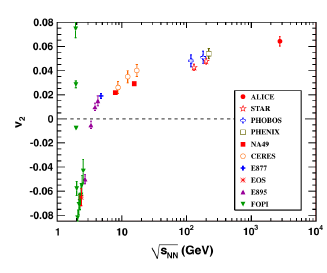
\includegraphics{elipFlow}
      \caption{ $v^{2}$ elliptical flow measurements from SPC to the LHC.}
      \label{fig:elipFlow}
    \end{figure}

     \begin{figure}[!Hhbt]
      \centering
      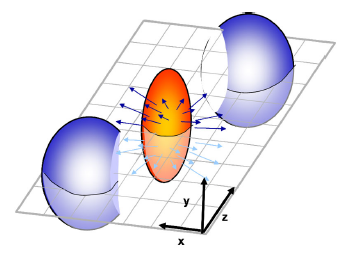
\includegraphics{elipFlowSchem}
      \caption{ Elliptical flow schematic diagram.}
      \label{fig:elipFlowSchem}
    \end{figure}

    \begin{figure}[!Hhbt]
      \centering
      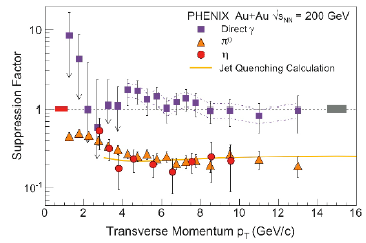
\includegraphics{hadRaaRhic}
      \caption{Hadron R$_{AA}$ from RHIC}
      \label{fig:hadRaaRhic}
    \end{figure}

    \begin{figure}[!Hhbt]
      \centering
      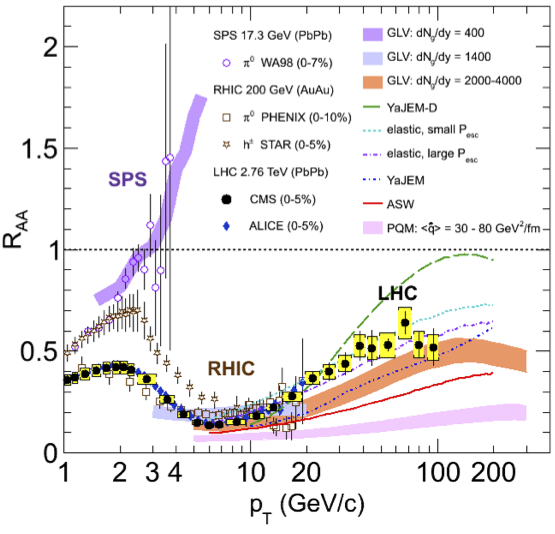
\includegraphics[width=.45\textwidth]{hadRaaLhc}
      \caption{Hadron R$_{AA}$ from the LHC.}
      \label{fig:hadRaaLhc}
    \end{figure}

    \begin{figure}[!Hhbt]
      \centering
      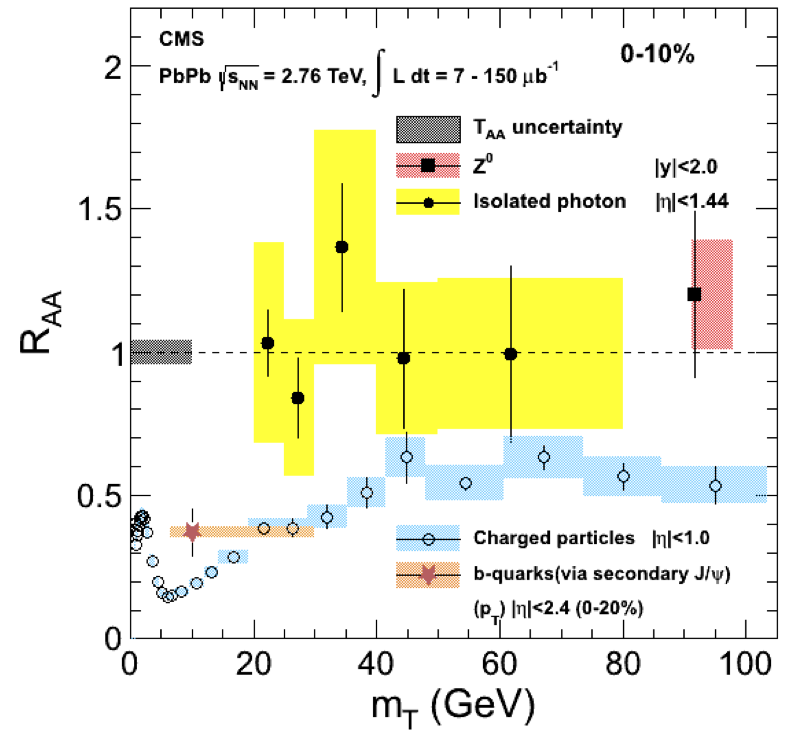
\includegraphics[width=.45\textwidth]{noRaaLhc}
      \caption{R$_{AA}$ for unsuppressed Z bosons and isolated photons.}
      \label{fig:noRaaLhc}
    \end{figure}

  \section{Recent results from HI control measurements}

    \subsection{The HI collision}
      The AGS and SPS created the first signs of a deconfined state, but the 
        nature of the state was uncertain.
      At RHIC the existence of the QGP was confirmed and it's nature found to 
        be hydrodynamic.
      The LHC and RHIC experiments are now looking deeper in the characteristics
        of QGP.
      More precise and sophisticated measurement techniques now require a 
        better understanding of the ions before they collide in order to 
        produce the proper theoretical modeling. 

      Over the course of the experimental evolution the following picture of 
        a heavy ion collision emerged. 
      First, highly contracted ions travel toward each other.
      Second, QGP forms and reaches thermal equilibrium.
      Third, this hot dense state expands hydrodynamically.
      Fifth, Fifth as the collection of quarks and gluons cool, a gas of hot
        hadrons forms and expands.
      Finally, all interactions freeze out and the produced particles stream 
        to the detector. 
